% !TeX encoding = UTF-8
% !TeX spellcheck = fr-classique
%%% DOCUMENTCLASS 
%%%-------------------------------------------------------------------------------

\documentclass[
  a4paper, % Format du papier
  11pt, extrafontsizes, % Taille des polices
  % oneside, 
  onecolumn, % Une colonne par page.
  openright, % Débuts de chapitres en recto.
]{memoir}
\usepackage{EcoFoG} % Modèle EcoFoG.sty

%% Options obligatoires pour la page de garde, package pdgUniv
% - DocType = HDR ou PhD
% - ED = UG ou UA (école doctorale, sans effet si DocType=HDR)
% - Ets = UG ou UA ou APT (établissement qui délivre le diplôme)
% - DIS = ST (Sciences et Technologies) ou SAN (Santé) ou ALL	(Arts, Lettres, Langues) 
%         ou DSE (Droit, Sciences Économiques et Gestion) ou SHS (Sciences Humaines et Sociales) 
% - ED2 (optionnel) = A (Cotutelle avec l'Université de A) ou B (à définir dans les futures versions)
% - emptypageafter : ajout d'une page blanche au verso de la page de garde
% - draft : pas de calcul de la page de garde pour gagner du temps à chaque compilation
\usepackage[DocType=PhD, ED=UG, Ets=UG, DIS=ST, emptypageafter]{pdgUniv}

%%% LOGOS 
%%%------------------------------------------------------------------------------
% Les fichiers Logo-Univ.pdf et Logo-Lab.pdf sont obligatoires
% Remplacer le logo d'EcoFoG par celui du labo du thésard, en le nommant Logo-Lab.pdf

%%% PACKAGES 
%%%------------------------------------------------------------------------------

% Ajouter ici les packages supplémentaires
% Attention, beaucoup sont déjà déclarés
%\usepackage{xxx}

%%% COMMANDS 
%%%------------------------------------------------------------------------------
% Césures particulières
\hyphenation{cé-su-re}
% Ajouter ici les commandes personnalisées
%\newcommand*{\xq}[6][]{{#1^{#3}_{#6}\!#2^{#4}_{#5}}}

%%% BIBLIOGRAPHY FILE
%%%------------------------------------------------------------------------------
\bibliography{library}
 
%%% THE DOCUMENT
%%%-------------------------------------------------------------------------------

%% Paramétrage de \makeflyleaf pour une thèse ou un mémoire d'HDR
%% Le code nécessaire est fourni par le package pdgUniv.sty 
% ==================
% Setup basic string
% - PhD Title
% - specialty: completes the dicipline passed as an argument to the pdgUniv package
% - author
% - defence date
% - laboratory
% - cotutelle
\specialty{\'Ecologie}
\title{Titre du mémoire, v.1.13, éventuellement très, très long et distribué sur plusieurs lignes}
\author{Auteur du mémoire}
\defencedate{20 mai 2017}
\lab{UMR \'Ecologie des Forêts de Guyane}
% ==================
% Setup people like your boss, the jury team and the referees
% - First you need to define how number they will be in each category
%   It is done with the commands \nboss{n}, \nreferee{n} and \njudge{n}.
%   You can define more people in each category than the number given 
%   but only the first "\npeople" will be print.
% - Then use the command \makesomeone{<category>}{<number>}{<name>}{<status>}{<other>}
%   where:
%     <category> should be select in ['boss', 'referee', 'judge']
%     <number>   is the rank for printing the person. 
%                Only number <= "\npeople" will be printed
%     <name>     First name and las name of the people
%     <status>   Is (s)he a "charg\'e de recher" ou un "professeur d'universit\'e"...
%     <other>    What ever string you want to add (laboratory, jury member place...).
%% Jury (supprimer les lignes en trop)
\njudge{7}
\makesomeone{judge}{1}{Premier MEMBRE}{Professeur d'Université}{Président du Jury}
\makesomeone{judge}{2}{Second MEMBRE}{Directeur de Recherche}{Membre du Jury}
\makesomeone{judge}{3}{Troisième MEMBRE}{Chargé de Recherche}{Membre du Jury}
\makesomeone{judge}{4}{Quatrième MEMBRE}{Chargé de Recherche}{Membre du Jury}
\makesomeone{judge}{5}{Ciquième MEMBRE}{Chargé de Recherche}{Membre du Jury}
\makesomeone{judge}{6}{Sixième MEMBRE}{Chargé de Recherche}{Directeur de Thèse}
\makesomeone{judge}{7}{Septième MEMBRE}{Chargé de Recherche}{Co-Directeur de Thèse}
%% Fin du paramétrage de la page de garde Thèse/HDR

%%%------------------------------------------------------------------------------
\begin{document}

%%----------------------------------
% knitr : décommenter ces lignes si le document est au format .Rnw et utilise knitr
% Réduction de l'espacement vertical entre le code R et les résultats produits par knitr
%\renewenvironment{knitrout}{\setlength{\topsep}{1mm}}{} 
%<<Declarations, echo=FALSE, include=FALSE>>=
%library(knitr)
%opts_knit$set(concordance=TRUE)
%# set global chunk options
%opts_chunk$set(cache=TRUE, warning=FALSE, tidy=TRUE, fig.width=8, fig.height=6, out.width='.8\\maxwidth', tidy.opts=list(keep.blank.line=FALSE, width.cutoff=60), size="scriptsize")
%options(width=60)
%par(mar=c(0,0,0,0))
%@
%%----------------------------------


% Langue
\selectlanguage{french}
% Affichage des nombres et unités (package SI) dans la même langue
\sisetup{locale = FR}

%%%------------------------------------------------------------------------------
\frontmatter

% Création de la couverture
\makeflyleaf


% Table des matières, marges étroites
\SmallMargins

\tableofcontents*
\clearpage

\LargeMargins

\chapter{Chapitre du préambule}

\lettrine{C}{e} chapitre peut être utilisé pour définir les notations, ou pour les remerciements. Exemple:

\noindent $A$: l'aire d'étude, et, selon le contexte, sa surface.



%%%------------------------------------------------------------------------------
\mainmatter
\LargeMargins                   % Délaration des marges larges



\chapter{Chapitre normal}

\lettrine{L}{e} texte respecte les standards de \LaTeX. 
Le modèle s'appuie le package \code{memoir}. 
La mise en page utilise intensivement les marges, pour les références bibliographiques, les légendes, les notes de bas de page (affichées en marge) et éventuellement les figures et tableau de petite taille. 
Les bas de page ne sont utilisés que pour le code informatique (par exemple l'affichage du code R utilisé pour créer les figures).


\section{Particularités du modèle}

Le modèle est prévu pour des documents longs (plusieurs chapitres), imprimés au format A4 en recto-verso.
Deux types de page de couverture sont disponible, pour une thèse ou un mémoire d'HDR. Le préambule du document est documenté pour passer d'un modèle à l'autre facilement. 

Il peut être utilisé pour la rédaction classique avec un éditeur \LaTeX ou dans R Studio pour l'utilisation de \code{knitr} ou \code{Sweave}:
\begin{itemize}
  \item l'extension du fichier doit être \code{.Rnw} au lieu de \code{.tex}
  \item les lignes de paramétrage (prévues pour \code{knitr}), tout au début du document, doivent être décommentées.
  \item le code R doit être saisi dans des bouts de code (\emph{\foreignlanguage{english}{code chunks}}). Le code peut être affiché ou non dans le document, et utilisé pour créer les figures à la volée. Le cache de \code{knitr} permet de ne pas reéxécuter tout le code à chaque compilation.
\end{itemize}


\subsection{Organisation du document}

Le document commence par un préambule (\code{\textbackslash frontmatter}) qui contient une page de titre formatée automatiquement à partir des informations saisies (auteur, titre et date), une deuxième page non modifiable, la table des matières (détaillée jusqu'au niveau sous-section) et éventuellement des chapitres non numérotés (remierciements, \dots). 
Le corps du document (\code{\textbackslash mainmatter}) contient les chapitres numérotés. 
La fin du document (\code{\textbackslash backmatter}) contient éventuellement des chapitres non numérotés (conclusion, post-face) et la bibliographie. 
Le document est imprimé en recto-verso avec les débuts de chapitre en pages impaires.

Les chapitres peuvent avoir des largeurs de marge différentes; normalement:
\begin{itemize}
  \item le préambule a des marges étroites (si les notes et références bibliographiques sont inutiles)
  \item le corps du document a des marges larges.
  \item la fin du document a des marges étroites.
\end{itemize}

\subsubsection{Hiérarchie des titres}

Le modèle s'appuie sur \code{memoir} qui gère les chapitres, sections (et sous-sections), paragraphes (et sous-paragraphes). 
Les titres du corps du document (\code{\textbackslash mainmatter}) sont numérotés jusqu'à la sous-section.

\subsubsection{Langues}

Le Français et l'Anglais sont supportés. 
La langue principale est déclarée normalement juste après le début du document. 
Le package \code{SI} est utilisé pour afficher les nombres et unités (par exemple \code{\textbackslash SI\{12\}\{\textbackslash kilo\textbackslash meter\textbackslash squared\}} pour afficher \SI{12}{\kilo\meter\squared}) et doit être paramétré dans la même langue. 
Il est possible de changer de langue en cours de document (changer en même temps le paramétrage de \code{babel} et \code{SI}). 
Pour un changement temporaire (par exemple un mot cité en Anglais), utiliser la commande \code{\textbackslash foreignlanguage\{english\}\{English word\}}) pour permettre la césure et le respect des normes typographiques.

\subsubsection{Figures et tableaux}

Les figures au format \code{eps}, \code{pdf}, \code{jpg} ou \code{png} doivent être placées dans le dossier \code{graphics}.

\figureSC{fig:sc}
  {Figure avec légende dans la marge (\code{\textbackslash figureSC})}
  {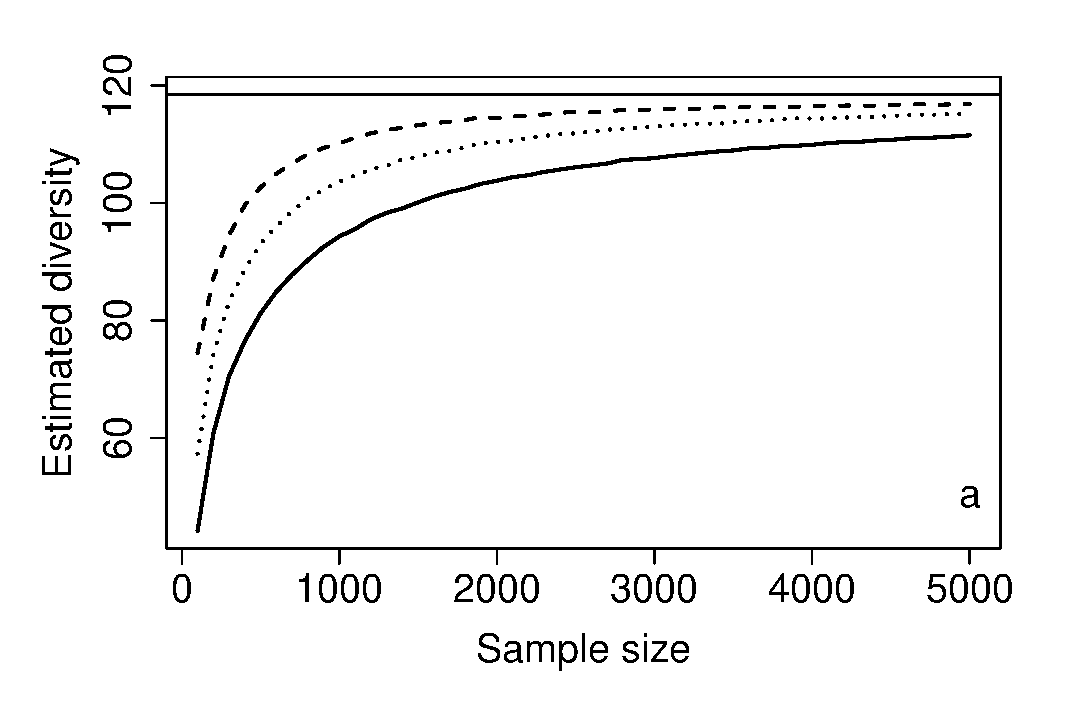
\includegraphics[width=.8\textwidth]{Fig1}}

Les tableaux et figures sont appelés par les commandes du type \code{\textbackslash tableSC}. Le préfixe est \code{table} ou \code{figure}; le suffixe peut être:
\begin{itemize}
  \item \code{SC} (figure~\ref{fig:sc}) pour \foreignlanguage{english}{Side Caption}: l'objet est placé dans le texte (sa largeur par défaut est 80\% de la largeur de la colonne), la légende est dans la marge. Le placement par défaut est \code{[htbp]}.

\tableFW{tab:FW}
{Notations des effectifs, tableau espèces-communautés.}
{
\begin{tabularx}{\textwidth}{p{2cm} p{7cm} p{1cm} X}
\toprule
 & Communauté $i$ & $\dots$ & Total: méta-communauté \\

\midrule
Espèce $s$ 
   & $n_{si}$: nombre d'individus de l'espèce $s$ dans la communauté $i$. \newline
  $\hat{p}_{si}=n_{si}/n_{+i}$ est l'estimateur de la probabilité $p_{si}$ qu'un individu de la communauté $i$ soit de l'espèce $s$.
  &
  & $n_{s+}=\sum_i{n_{si}}$ \newline
    $p_s=\sum_i{w_{i}p_{si}}$ \\

$\dots$
  &
  &
  & \\

Total
  & $n_{+i}$: nombre d'individus de la communauté.\newline 
    $w_i$: poids de la communauté
  &
  & $n$: nombre total d'individus échantillonnés \\

\bottomrule
\end{tabularx}
}

  \item \code{FW} (tableau~\ref{tab:FW}) pour \foreignlanguage{english}{Full Width}: l'objet occupe toute la largeur de la page (hors marges d'impression), la légende est dans le texte, au dessus pour les tableaux, au-dessous pour les figures. Le placement par défaut est \code{[tbp]}.

\figureMargin{fig:Margin}
  {Figure dans la marge (\code{\textbackslash figureMargin})}
  {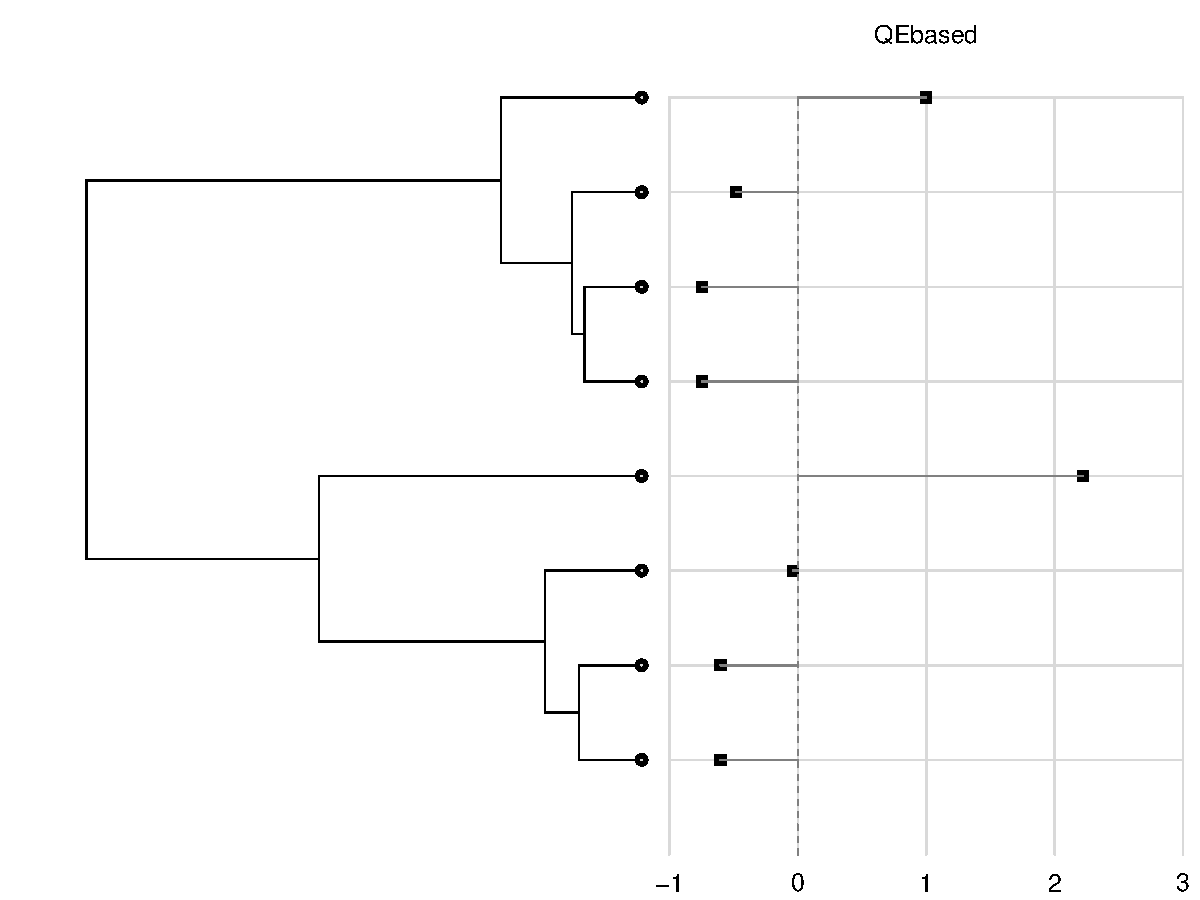
\includegraphics[width=\textwidth]{Fig2}}

  \item  \code{Margin} (figure~\ref{fig:Margin}) pour placer l'objet et sa légende dans la marge.
\end{itemize}

\figureFW{fig:subfig}
{Figure multiple. La commande \code{\textbackslash includegraphics} est simplement remplacée par les commandes \code{\textbackslash subfloat}}
{
  \subfloat[Première sous figure. \label{fig:subfiga}]
    {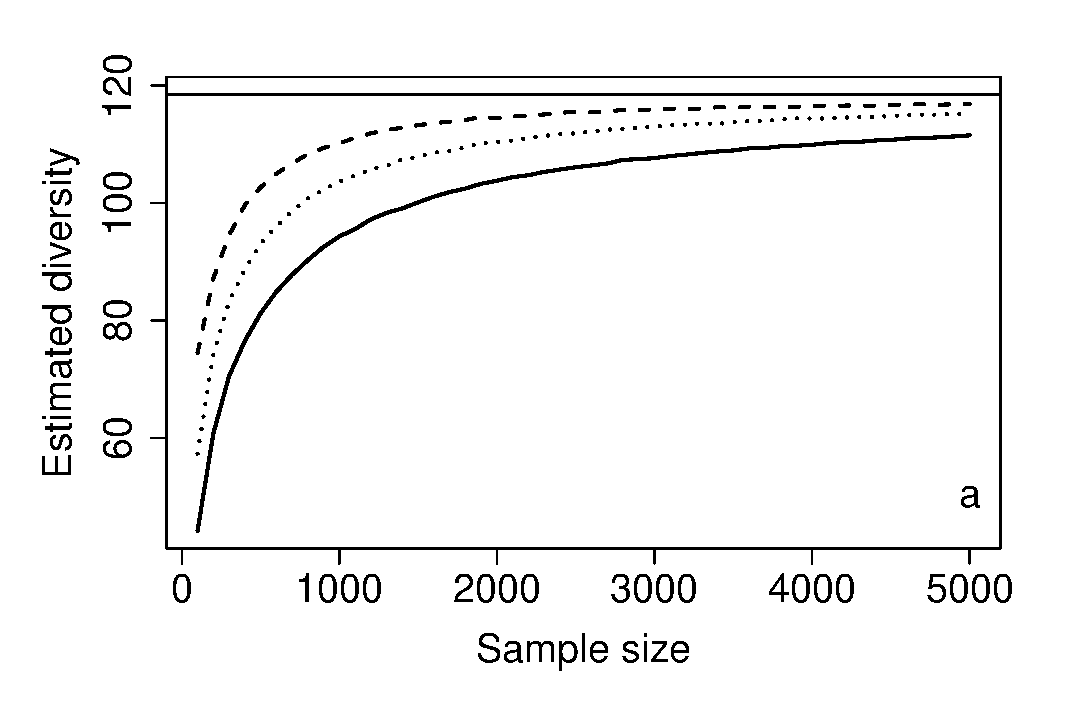
\includegraphics[width=.45\textwidth]{Fig1}}
	\hfill
  \subfloat[Deuxième sous figure. \label{fig:subfigb}]
    {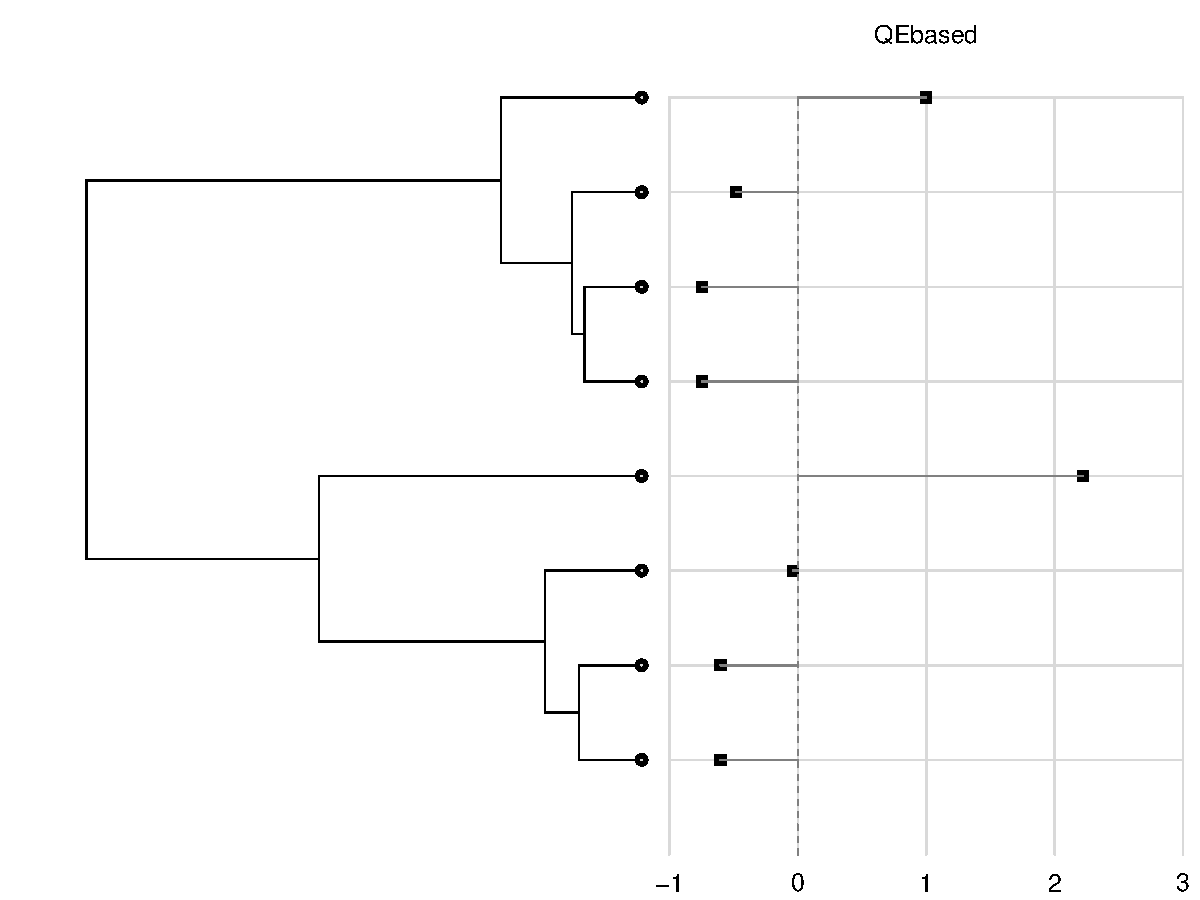
\includegraphics[width=.45\textwidth]{Fig2}}
}

La syntaxe des six commandes est identique, avec 4 paramètres dont trois obligatoires:
\begin{itemize}
  \item paramètre optionnel (ignoré pour les objets dans la marge): placement, par défaut \code{[htbp]} ou \code{[tbp]}.
  \item étiquette de l'objet.
  \item légende
  \item contenu de l'objet, en général un tableau, \code{\textbackslash includegraphics} ou un bout de code R si \code{knitr} est utilisé. Le package \code{subfig} permet des figures multiples (figure~\ref{fig:subfig}), de préférence en pleine largeur.
\end{itemize}


\subsection{Notes}

Les notes sont appelées par \code{\textbackslash footnote} mais sont affichées en marge\footnote{Exemple de note de \og bas de page\fg{}}.

Le code informatique utilisé dans des bouts de code R (\foreignlanguage{english}{\emph{chunks}}) peut être placé en bas de page en utilisant \code{\textbackslash verbfootnote} \verbfootnote{
\scriptsize
Code R:

> 2+2

[1] 4
}
.


\section{Commandes}

\subsection{Nouvelles commandes}

Les nouvelles commandes suivantes sont incluses dans le modèle:
\begin{itemize}
  \item \code{\textbackslash Var} pour la variance, en mode mathématique: $\Var(X)=\nicefrac{\sum_i(x_i-\bar{x})^2}{(n-1)}$,
  \item \code{\textbackslash code\{\}} pour afficher du code dans le texte. Attention, le code est insécable et peut provoquer des dépassements de largeur de ligne (\foreignlanguage{english}{``Overfull hbox''}) si leur retour à la ligne cause un espacement trop important entre les mots. Forcer dans ce cas le retour à la ligne en insérant \code{\textbackslash break} avant le code.
\end{itemize}

\subsection{\'Equations}

Utiliser les environnements \code{\textbackslash equation} ou \code{\textbackslash multline}:

\begin{multline}
  \tilde{H}
  = -\sum_{s=1}^{s^{n}_{\ne 0}}
    {\frac{n_s}{n}\left(\mathrm{\Psi}\left(n\right) - \mathrm{\Psi}\left(n_s\right)\right)} \\
    -\frac{s_{1}}{n} {\left(1-A\right)}^{1-n} \left(-{\ln\left(A\right)}-\sum^{n-1}_{r=1}{\frac{1}{r}{\left(1-A\right)}^r}\right)
\label{eq:Chao2013}
\end{multline}

 \code{\textbackslash align} permet de présenter les calculs en plusieurs lignes:

\begin{align}
  ^{q}\bar{H}_{\beta}\left(T\right)
    &= \sum_i{w_i}\sum_k{\frac{T_k}{T}{^{q}_{ik}H}}\\
    &= \sum_i{w_i}\sum_k{\frac{T_k}{T}\sum_u{p^{q}_{kui}\ln_q\frac{p_{kui}}{p_{ku}}}}
\end{align}



\section{Bibliographie}

Les références bibliographiques doivent être appelées par la commande \code{\textbackslash autocite}. 
Elles sont affichées en marge \autocite{Rao1985} et dans le récapitulatif en fin de document.
Si le DOI est renseigné dans la base bibliographique, il est affiché sous la forme d'un lien hypertexte qui permet d'accéder directement à la référence en ligne.
La commande \code{\textbackslash textcite} permet d'intégrer le nom des auteurs dans le texte, par exemple: \textcite{Rao1985}.

Les références répétées \autocite{Pelissier2001} sont traitées.
Une répétition immédiate est remplacée par \emph{Ibid.} \autocite{Pelissier2001}
Une répétition sur la même (double) page séparée par une autre citation \autocite{Rao1985} est réduite au nom de l'auteur et à l'année \autocite{Pelissier2001}.
Une répétition au delà de la double page affiche en plus le titre et un renvoi vers la page de la première citation.

La bibliographie est gérée par \code{biblatex}.
Elle peut être imprimée sur une ou deux colonnes, selon sa longueur.




\chapter{Disciplines et spécialités}

La discipline et la spécialité du doctorat ou de l’HDR doivent être choisies dans les listes ci-dessous.
La liste des disciplines est limitative: le choix de la discipline est une option du package \code{pdgUniv} dans l'entête de ce document. 
La liste des spécialités peut être complétée sur demande à l’École doctorale: la spécialité est saisie librement dans la variable \code{specialty} dans l'entête de ce document.
La liste actuelle est fournie ici.

\section{Sciences et Technologies}

\begin{itemize}
  \item Aspects moléculaires et cellulaires de la biologie
  \item Physiologie et biologie des organismes-populations-interactions
  \item Sciences de la vie
  \item Sciences de l’environnement
  \item Sciences de la terre
  \item Génétique 
  \item Biologie
  \item Écologie
  \item Hydrologie
  \item Sciences agronomiques, biotechnologies agro-alimentaires 
  \item Géosciences
  \item Chimie 
  \item Chimie des substances naturelles
  \item Physique
  \item Génie civil 
  \item Mathématiques 
  \item Informatique
  \item Électronique
  \item Génie électrique 
  \item Génie des procédés
  \item Sciences et technologie industrielles 
  \item Sciences de la matière
\end{itemize}	


\section{Santé}

\begin{itemize}
  \item Médecine
  \item Recherche clinique, innovation technologique, santé publique 
\end{itemize}	


\section{Arts, Lettres, Langues}

\begin{itemize}
  \item Arts et études cinématographiques et audiovisuelles
  \item Littérature générale comparée
  \item Cultures et langues régionales 
  \item Langues et littératures anciennes 
  \item Langues et littératures étrangères 
  \item Langues et littératures françaises 
  \item Langues étrangères appliquées 
  \item Sciences du langage 
  \item Sciences du langage – Français langue étrangère
\end{itemize}	


\section{Droit, Sciences Économiques et Gestion}

\begin{itemize}
  \item Sciences juridiques - Droit public
  \item Sciences juridiques - Droit privé 
  \item Sciences juridiques - Droit des affaires
  \item Sciences politiques 
  \item Sciences économiques
  \item Sciences de gestion
\end{itemize}	


\section{Sciences Humaines et Sociales}

\begin{itemize}
  \item Archéologie, ethnologie, préhistoire 
  \item Ethnologie/anthropologie
  \item Aménagement
  \item Histoire
  \item Géographie
  \item Sciences de l’éducation
  \item Sciences de l’information et de la communication
  \item Sociologie
  \item Sociologie, démographie
\end{itemize}	




% Marges étroites
\clearpage
\SmallMargins
\chapter{Mise en page alternative}

Une autre mise en page possible utilise des marges étroites.
Elle est déconseillée parce que moins lisible : chaque ligne contient une centaine de caractères, bien au-delà des 60 caractères optimaux pour la lecture.
Les bas de page sont utilisés pour toutes les notes.


\section{Figures et tableaux}


\figureFW{fig:FW}
{Figure avec légende (\code{\textbackslash figureFW})}
{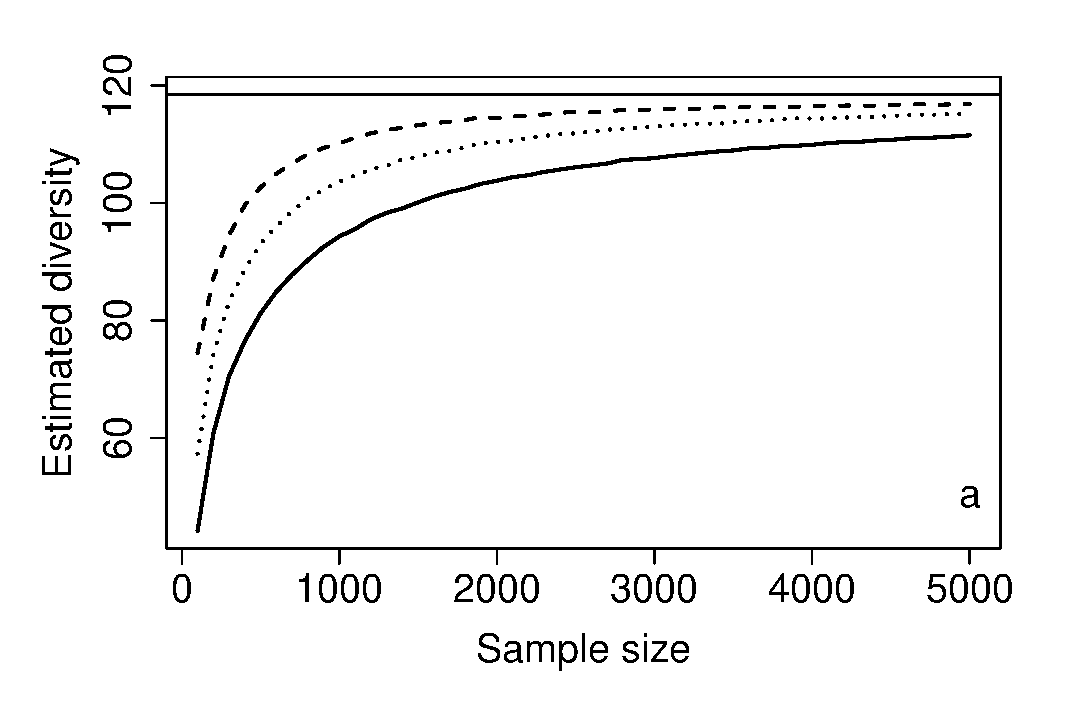
\includegraphics[width=.8\textwidth]{Fig1}}

Les tableaux et figures sont appelés par les seules commandes \code{\textbackslash tableFW} et \code{\textbackslash figureFW}; les autres suffixes ne sont pas utilisables avec les marges étroites, faute de place.
L'objet occupe toute la largeur de la page (hors marges d'impression), la légende est dans le texte, au dessus pour les tableaux, au-dessous pour les figures. Le placement par défaut est \code{[tbp]}.


\section{Notes}

Les notes sont appelées par \code{\textbackslash footnote}\footnote{Exemple de note de bas de page}.

Le code informatique utilisé dans des bouts de code R (\foreignlanguage{english}{\emph{chunks}}) peut être placé en bas de page en utilisant \code{\textbackslash verbfootnote} \verbfootnote{
  \scriptsize
  Code R:
  
  > 2+2
  
  [1] 4
}
.


\section{Bibliographie}

Les références bibliographiques doivent être appelées par la commande \code{\textbackslash autocite}. 
Elles sont affichées en bas de page \autocite{Rao1985} et dans le récapitulatif en fin de document.
La commande \code{\textbackslash textcite} permet d'intégrer le nom des auteurs dans le texte, par exemple: \textcite{Rao1985}.

Les références répétées \autocite{Pelissier2001} sont traitées.
Une répétition immédiate est remplacée par \emph{Ibid.} \autocite{Pelissier2001}
Une répétition sur la même (double) page séparée par une autre citation \autocite{Rao1985} est réduite au nom de l'auteur et à l'année \autocite{Pelissier2001}.
Une répétition au delà de la double page affiche en plus le titre et un renvoi vers la page de la première citation.

La bibliographie est gérée par \code{biblatex}.
Elle peut être imprimée sur une ou deux colonnes, selon sa longueur.



%%%------------------------------------------------------------------------------
\backmatter
\clearpage

%%% BIBLIOGRAPHY
%%% -------------------------------------------------------------

% Marges étroites
\SmallMargins

% Si la bilbiographie est longue, police plus petite et deux colonnes (décommenter les deux lignes)
%\twocolumn
%\renewcommand*{\bibfont}{\scriptsize}

\printbibliography

\end{document}
